\documentclass[../Document.tex]{subfiles}
\graphicspath{{\subfix{../images/}}}

\begin{document}


\section{Constraint Programming}
\label{sec:intro/cp}
\acrlong{cp} is a complete, heuristic guided search method which excels at ensuring the respect of constraints while generating a solution. It is complete in that if a solution exists in a given search space, a \gls{cp} model is guaranteed to find it. By using heuristics as well as constraint propagation (more on that later), it can be much faster than a simple brute force of all possible solutions.

% We will first define how a simple \gls{cp} model functions: its definition, the declaration of constraints, the constraint propagation, the branching decisions, error detection and management.
We will first define how a simple \gls{cp} model functions. We will cover the initial problem declaration, the constraint declaration to describe the problem and finally the solving process and its intricacies (constraint propagation, branching decisions, backtracking).
Once that is covered, we can expand on this topic by introducing \gls{cpbp}
\david{cite BP from original paper}
which is an improvement over standard constraint propagation and leads to more informed decisions. We use \gls{cpbp} in our work since it tends to yield better results and allows for the combination with a \gls{ml} model as we will describe later.

%%% SubSection Base Model Definition %%%
\subsection{Constraint Satisfaction Problem}
A \gls{csp} is defined in three parts:
\begin{itemize}
    \item The variables making up the problem, defined as the finite set $\mathcal{X}$
    \item The domains of these variables, defined as a finite set of values $D$. Each variable can have its own domain
    \item The constraints, each of which is applied to a subset of the variables, defined as a set of constraints $C$.
\end{itemize}

There are a finite number of \textbf{variables} defined in the set $\mathcal{X}$. Each of these variables has its own \textbf{domain} as is defined in the set $D$, which contains the possible values that a variable may take on. Finally, we define a finite number of \textbf{constraints}, each of which is applied on a subset of the variables. Each variable must then be assigned a value from its domain such that it respects all the applied constraints. If such an assignment is possible for all the variables, that is a solution to the problem.

If we take the Sudoku problem as an example, a classic and very commonly seen problem, we can define it as a \gls{csp} as follows.
Our \textbf{variables} will be each tile in the 9x9 grid. While this gives us the layout of our problem, we must define the possible values for each variable to be able to solve this problem.
All the variables can take on the same values and so we can define the \textbf{domain} as being the integer values between 1 and 9 inclusively. 

We could represent this using a 2-dimensional array of variables like so:

\begin{align}
    tile[i][j] \in \{1,2,\dots,9\} \mid i,j \in \{1,2,\dots,9\}
\end{align}

All that is missing are the constraints, which are the source of the complexity of the problem.

The \textbf{constraints} in a Sudoku are fairly straightforward, lines, columns and all 3x3 sub-grids within the total grid may not contain any repeat values.
In the \gls{cp} community, this type of constraint is very common and is called an \texttt{alldifferent} constraint. The Sudoku problem would therefore have the following constraints:

\begin{gather*}
    \texttt{alldifferent}(tile[1][j], tile[2][j], \dots, tile[9][j])\ \forall\ j \mid j \in \{1,2,\dots,9\} \\
    \texttt{alldifferent}(tile[i][1], tile[i][2], \dots, tile[i][9])\ \forall\ i \mid i \in \{1,2,\dots,9\} \\
    \texttt{alldifferent}(\\
        tile[3u+1][3v+1],tile[3u+1][3v+2],tile[3u+1][3v+3],\\
        tile[3u+2][3v+1],tile[3u+2][3v+2],tile[3u+2][3v+3],\\
        tile[3u+3][3v+1],tile[3u+3][3v+2],tile[3u+3][3v+3],\\
    )\ \forall\ u,v \mid u,v \in \{0,1,2\}
\end{gather*}

Overall, we would need 81 variables to define this \gls{csp} as well as 27 constraints. Each of our variables could take on any of the 9 possible values in their domain.

%%% SubSection Domain Filtering %%%
\subsection{Domain Filtering}
As mentioned in the previous section, each constraint is applied to a subset of the variables in the problem definition. When a constraint is declared, a filtering algorithm that is specific to that constraint will eliminate values that are inconsistent.

The simple example below illustrates how a constraint can filter a variable's domain after being declared.

\begin{gather*}
    x \in \{2,3,4\}\\
    y \in \{1,2,3\}\\
    x \leq y\\
    x \in \{2,3,\bcancel{4}\}\\
    y \in \{\bcancel{1},2,3\}
\end{gather*}

Both variables initially contained a value that would always breach the constraint if chosen. A value such as that one is said to have no support, \ie there are no solutions to the current constraint that contain this value. A visual representation of this can be seen in Figure~\ref{fig:domain_filtering}, where a constraint is applied to two different variables and both have their domain filtered. While we do not know all the solutions to a problem in all cases, we can use logical processes to determine values that would guarantee a breach of the constraint.


\begin{figure}[ht]
    \centering
    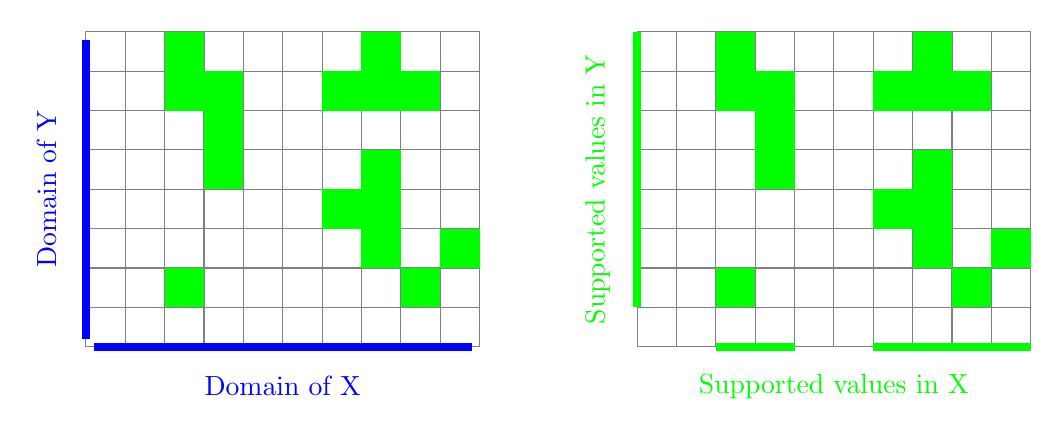
\begin{tikzpicture}
    \def\size{0.5}
    \def\columns{10}
    \pgfmathtruncatemacro{\lastCol}{\columns - 1}
    \def\rows{8}
    \pgfmathtruncatemacro{\lastRow}{\rows - 1}

    \foreach \x in {0,...,\lastCol} {
        \foreach \y in {0,...,\lastRow} {
            \draw[gray] 
            ({\x * \size}, {\y * \size})
            rectangle ++(\size,\size);
        }
    }
    
    % Row 2
    \foreach \x in {2,8} {
        \fill[green]
            ({\x * \size},{1 * \size})
            rectangle ++(\size,\size);
    }
    
    % Row 3
    \foreach \x in {7,9} {
        \fill[green]
            ({\x * \size},{2 * \size})
            rectangle ++(\size,\size);
    }
    
    % Row 4
    \foreach \x in {6,7} {
        \fill[green]
            ({\x * \size},{3 * \size})
            rectangle ++(\size,\size);
    }
    
    % Row 5
    \foreach \x in {3,7} {
        \fill[green]
            ({\x * \size},{4 * \size})
            rectangle ++(\size,\size);
    }

    % Row 6
    \fill[green]
        ({3 * \size},{5 * \size})
        rectangle ++(\size,\size);
    
    % Row 7
    \foreach \x in {2,3,6,7,8} {
        \fill[green]
            ({\x * \size},{6 * \size})
            rectangle ++(\size,\size);
    }

    % Row 8
    \foreach \x in {2,7} {
        \fill[green]
            ({\x * \size},{7 * \size})
            rectangle ++(\size,\size);
    }

    % Bottom border
    \node[text=blue] at ({(10*\size)/2}, -0.5) {Domain of X};
    \draw[line width=3pt, blue]
        (0.2 * \size, 0)
        -- ++(9.6 * \size, 0);

    % Left border
    \node[text=blue, rotate=90] at (-0.5, {(8*\size)/2}) {Domain of Y};
    \draw[line width=3pt, blue]
        (0, 0.2 * \size)
        -- ++(0, 7.6 * \size);
    
    \begin{scope}[shift={({\columns*\size + 2}, 0)}]
        \foreach \x in {0,...,\lastCol} {
            \foreach \y in {0,...,\lastRow} {
                \draw[gray] 
                ({\x * \size}, {\y * \size})
                rectangle ++(\size,\size);
            }
        }

        % Row 2
        \foreach \x in {2,8} {
            \fill[green]
                ({\x * \size},{1 * \size})
                rectangle ++(\size,\size);
        }
        
        % Row 3
        \foreach \x in {7,9} {
            \fill[green]
                ({\x * \size},{2 * \size})
                rectangle ++(\size,\size);
        }
        
        % Row 4
        \foreach \x in {6,7} {
            \fill[green]
                ({\x * \size},{3 * \size})
                rectangle ++(\size,\size);
        }
        
        % Row 5
        \foreach \x in {3,7} {
            \fill[green]
                ({\x * \size},{4 * \size})
                rectangle ++(\size,\size);
        }

        % Row 6
        \fill[green]
            ({3 * \size},{5 * \size})
            rectangle ++(\size,\size);
        
        % Row 7
        \foreach \x in {2,3,6,7,8} {
            \fill[green]
                ({\x * \size},{6 * \size})
                rectangle ++(\size,\size);
        }

        % Row 8
        \foreach \x in {2,7} {
            \fill[green]
                ({\x * \size},{7 * \size})
                rectangle ++(\size,\size);
        }

        % Bottom border
        \node[text=green] at ({(10*\size)/2}, -0.5) {Supported values in X};
        \draw[line width=3pt, green]
            (2 * \size, 0)
            -- ++(2 * \size, 0);
        \draw[line width=3pt, green]
            (6 * \size, 0)
            -- ++(4 * \size, 0);

        % Left border
        \node[text=green, rotate=90] at (-0.5, {(8*\size)/2}) {Supported values in Y};
        \draw[line width=3pt, green]
            (0, 1 * \size)
            -- ++(0, 7 * \size);
    \end{scope}
\end{tikzpicture}
    \caption[Domain filtering on one variable.]{A constraint is declared on both variable $X$ and $Y$. Valid combinations to the constraint are illustrated by green points on the grid. Values that have no support (no solution to this constraint contains these values) are removed from the domain of the variable. This can be seen as a projection of the solution space onto the domain of each variable.}
    \label{fig:domain_filtering}
\end{figure} 

%%% SubSection Constraint Propagation %%%
\subsection{Constraint Propagation}
Now that we have declared our constraints, the solver begins propagating the consequences of these constraints. Each constraint in the queue communicates to the variables it affects which values in the domain have to be filtered out. Once a variable's domain has been changed, it notifies the constraints that are affected by the change and those constraints are then added to the queue again.

The solver continues propagating the consequences of the constraints and updating domains until it reaches one of three situations: 
\begin{enumerate}
    \item The queue is empty, but there remain unassigned variables.
    \item All variables have been assigned a value, this is a solution to the problem.
    \item One of the variables' domain has been completely filtered, there is no solution in the current state of the problem.
\end{enumerate}

In the first case, there is nothing else to deduce with the information currently available and the solver has to make a branching decision from the current state. Any time we reach one of the three cases above, we can consider that state as being a node in the search tree. The solver makes a branching decision from the current node and propagates the consequences of this decision until it reaches another node to handle.

In the second case, the solver has found a solution and can add it it the solution set. Once the solution has been found, we backtrack to the previous node in the search tree and search along the other branches.

Finally, if we reach an unsatisfiable state, the solver backtracks to the previous node and continues its search from there.

Since we have a finite number of values, we know that this process will eventually end and we will either find a value that respects the constraint, or, find that the constraint cannot be satisfied.

To continue with the example of a Sudoku, a classic way humans continue solving, once they reach a dead end in their reasoning, is by assigning a value to a tile and seeing if they reach a contradictory state.
If they do, then they know their choice was wrong and they can eliminate that possibility.


%%% SubSection Marginal %%%
\subsection{Marginals-Augmented Constraint Programming}
In an ideal world, if we knew every possible solution to a problem, we could use the values within the solution to inform our search and avoid bad branching decisions. This is especially useful when we consider bigger problems that might have a huge combinatorial space to explore.

Marginals-augmented constraint programming is the idea of guiding our branching decisions by counting the number of solutions to a constraint that contain a given value for a given variable as seen in Figure~\ref{fig:marginal_cp}. The difficulty of this task is that it requires an efficient algorithm which can predict the number of solutions without finding and enumerating all possible solutions to the constraint.

\begin{figure}[ht]
    \centering
    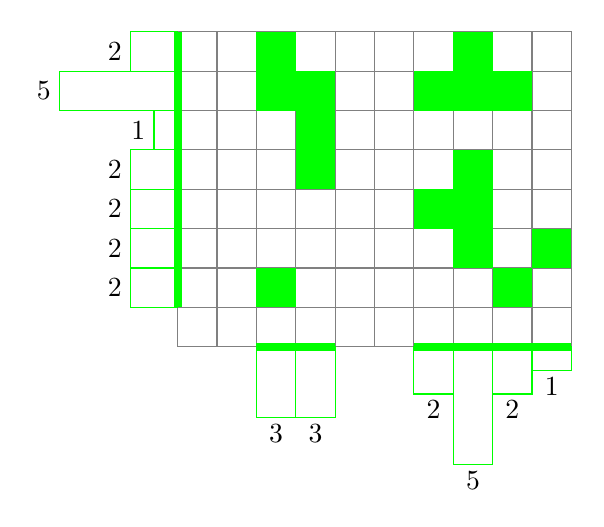
\begin{tikzpicture}
    \def\size{0.5}
    \def\columns{10}
    \pgfmathtruncatemacro{\lastCol}{\columns - 1}
    \def\rows{8}
    \pgfmathtruncatemacro{\lastRow}{\rows - 1}

    \foreach \x in {0,...,\lastCol} {
        \foreach \y in {0,...,\lastRow} {
            \draw[gray] 
            ({\x * \size}, {\y * \size})
            rectangle ++(\size,\size);
        }
    }
    
    % Row 2
    \foreach \x in {2,8} {
        \fill[green]
            ({\x * \size},{1 * \size})
            rectangle ++(\size,\size);
    }
    
    % Row 3
    \foreach \x in {7,9} {
        \fill[green]
            ({\x * \size},{2 * \size})
            rectangle ++(\size,\size);
    }
    
    % Row 4
    \foreach \x in {6,7} {
        \fill[green]
            ({\x * \size},{3 * \size})
            rectangle ++(\size,\size);
    }
    
    % Row 5
    \foreach \x in {3,7} {
        \fill[green]
            ({\x * \size},{4 * \size})
            rectangle ++(\size,\size);
    }

    % Row 6
    \fill[green]
        ({3 * \size},{5 * \size})
        rectangle ++(\size,\size);
    
    % Row 7
    \foreach \x in {2,3,6,7,8} {
        \fill[green]
            ({\x * \size},{6 * \size})
            rectangle ++(\size,\size);
    }

    % Row 8
    \foreach \x in {2,7} {
        \fill[green]
            ({\x * \size},{7 * \size})
            rectangle ++(\size,\size);
    }

    % Bottom border
    \node[text=green] at ({(10*\size)/2}, -0.5) {};
    \draw[line width=3pt, green]
        (2 * \size, 0)
        -- ++(2 * \size, 0);
    \draw[line width=3pt, green]
        (6 * \size, 0)
        -- ++(4 * \size, 0);

    % Left border
    \node[text=green, rotate=90] at (-0.5, {(8*\size)/2}) {};
    \draw[line width=3pt, green]
        (0, 1 * \size)
        -- ++(0, 7 * \size);

    % Left boxes
    \def\barSize{0.3}
    \foreach \marginal [count=\i from 1] in {2,2,2,2,1,5,2} {
        \draw[green] (0, \i * \size) rectangle ++(-\marginal * \barSize, 1*\size);
        \node at (-\marginal * \barSize - 0.2, \i * \size + 0.5 * \size) {\marginal};
    };
    
    % Bottom boxes
    \foreach \marginal [count=\i from 2] in {3,3} {
        \draw[green] (\i * \size, 0) rectangle ++(1*\size, -\marginal * \barSize);
        \node at (\i * \size + 0.5 * \size, -\marginal * \barSize - 0.2) {\marginal};
    };
    \foreach \marginal [count=\i from 6] in {2,5,2,1} {
        \draw[green] (\i * \size, 0) rectangle ++(1*\size, -\marginal * \barSize);
        \node at (\i * \size + 0.5 * \size, -\marginal * \barSize - 0.2) {\marginal};
    };

\end{tikzpicture}
    \caption[Marginal-Augmented \acrlong{cp}.]{Taking the same example as in Figure~\ref{fig:domain_filtering}, we can count how many valid solutions contain a given value for both variables $X$ and $Y$. The numbers seen on the left and the bottom of the grid indicate the number of solutions containing the value. This can help guide our branching decisions towards solution-dense regions in the search space.}
    \label{fig:marginal_cp}
\end{figure}

%%% SubSubSection CPBP %%%
% \subsubsection{Constraint Programming with Belief Propagation}
One use of these marginals is to change standard constraint propagation to contain more information. Belief Propagation does this by modifying the message that constraints send variables. Instead of sending a message containing a binary representation of which values in the domain have a support, the messages are modified to communicate the probability of a value being contained within a solution as seen in Figure~\ref{fig:cpbp_messaging}. This allows the solver to avoid branching on values that have a very small chance of being valid.




\begin{figure}[ht]
    \centering
    \vspace{0.5cm}
    \vbox to 4cm {
        
% region CPBP bar graphs

% Bar graph representing the blue constraint's marginals on variable x
\newcommand{\blueGraphX}{
    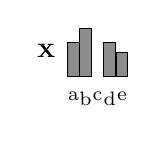
\begin{tikzpicture}
        \begin{axis}[
            ybar,
            axis y line=none,
            axis x line=bottom,
            axis line style={draw=none},
            ymin=0,
            ymax=100,
            width=2.2cm,
            height=2.2cm,
            bar width=1.5mm,
            xtick={a,b,c,d,e},
            xtick style={draw=none},
            symbolic x coords={a,b,c,d,e},
            xticklabel style={font=\scriptsize, anchor=north, yshift=-2pt},
            axis x line=bottom,
            axis y line=left,
            tick align=inside,
            enlarge x limits=0,
            clip=false,
        ]
            \addplot+[fill=gray!90, draw=black] coordinates {
                (a,70) (b,100) (d,70) (e,50)
            };
            \node[
                anchor=south east,
                font=\scriptsize\bfseries,
                xshift=-1mm, yshift=-5mm
            ] at (current axis.north west) {X};
        \end{axis}
    \end{tikzpicture}
}

% Bar graph representing the blue constraint's marginals on variable y
\newcommand{\blueGraphY}{
    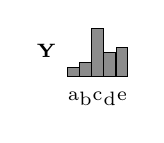
\begin{tikzpicture}
        \begin{axis}[
            ybar,
            axis y line=none,
            axis x line=bottom,
            axis line style={draw=none},
            ymin=0,
            ymax=100,
            width=2.2cm,
            height=2.2cm,
            bar width=1.5mm,
            xtick={a,b,c,d,e},
            xtick style={draw=none},
            symbolic x coords={a,b,c,d,e},
            xticklabel style={font=\scriptsize, anchor=north, yshift=-2pt},
            axis x line=bottom,
            axis y line=left,
            tick align=inside,
            enlarge x limits=0,
            clip=false,
        ]
            \addplot+[fill=gray!90, draw=black] coordinates {
                (a,20) (b,30) (c,100) (d,50) (e,60)
            };
            \node[
                anchor=south east,
                font=\scriptsize\bfseries,
                xshift=-1mm, yshift=-5mm
            ] at (current axis.north west) {Y};
        \end{axis}
    \end{tikzpicture}
}

% Bar graph representing the blue constraint's marginals on variable z
\newcommand{\blueGraphZ}{
    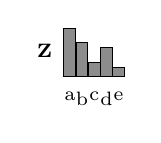
\begin{tikzpicture}
        \begin{axis}[
            ybar,
            axis y line=none,
            axis x line=bottom,
            axis line style={draw=none},
            ymin=0,
            ymax=100,
            width=2.2cm,
            height=2.2cm,
            bar width=1.5mm,
            xtick={a,b,c,d,e},
            xtick style={draw=none},
            symbolic x coords={a,b,c,d,e},
            xticklabel style={font=\scriptsize, anchor=north, yshift=-2pt},
            axis x line=bottom,
            axis y line=left,
            tick align=inside,
            enlarge x limits=0,
            clip=false,
        ]
            \addplot+[fill=gray!90, draw=black] coordinates {
                (a,100) (b,70) (c,30) (d,60) (e,20)
            };
            \node[
                anchor=south east,
                font=\scriptsize\bfseries,
                xshift=-1mm, yshift=-5mm
            ] at (current axis.north west) {Z};
        \end{axis}
    \end{tikzpicture}
}

% Bar graph representing the red constraint's marginals on variable x
\newcommand{\redGraphX}{
    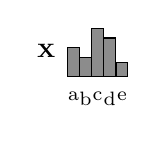
\begin{tikzpicture}
        \begin{axis}[
            ybar,
            axis y line=none,
            axis x line=bottom,
            axis line style={draw=none},
            ymin=0,
            ymax=100,
            width=2.2cm,
            height=2.2cm,
            bar width=1.5mm,
            xtick={a,b,c,d,e},
            xtick style={draw=none},
            symbolic x coords={a,b,c,d,e},
            xticklabel style={font=\scriptsize, anchor=north, yshift=-2pt},
            axis x line=bottom,
            axis y line=left,
            tick align=inside,
            enlarge x limits=0,
            clip=false,
        ]
            \addplot+[fill=gray!90, draw=black] coordinates {
                (a,60) (b,40) (c,100) (d,80) (e,30)
            };
            \node[
                anchor=south east,
                font=\scriptsize\bfseries,
                xshift=-1mm, yshift=-5mm
            ] at (current axis.north west) {X};
        \end{axis}
    \end{tikzpicture}
}

% Bar graph representing the red constraint's marginals on variable w
\newcommand{\redGraphW}{
    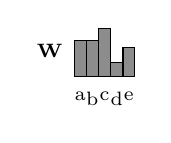
\begin{tikzpicture}
        \begin{axis}[
            ybar,
            axis y line=none,
            axis x line=bottom,
            axis line style={draw=none},
            ymin=0,
            ymax=100,
            width=2.2cm,
            height=2.2cm,
            bar width=1.5mm,
            xtick={a,b,c,d,e},
            xtick style={draw=none},
            symbolic x coords={a,b,c,d,e},
            xticklabel style={font=\scriptsize, anchor=north, yshift=-2pt},
            axis x line=bottom,
            axis y line=left,
            tick align=inside,
            enlarge x limits=0,
            clip=false,
        ]
            \addplot+[fill=gray!90, draw=black] coordinates {
                (a,75) (b,75) (c,100) (d,30) (e,60)
            };
            \node[
                anchor=south east,
                font=\scriptsize\bfseries,
                xshift=-1mm, yshift=-5mm
            ] at (current axis.north west) {W};
        \end{axis}
    \end{tikzpicture}
}

% Bar graph representing the red constraint's marginals on variable z
\newcommand{\redGraphZ}{
    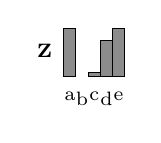
\begin{tikzpicture}
        \begin{axis}[
            ybar,
            axis y line=none,
            axis x line=bottom,
            axis line style={draw=none},
            ymin=0,
            ymax=100,
            width=2.2cm,
            height=2.2cm,
            bar width=1.5mm,
            xtick={a,b,c,d,e},
            xtick style={draw=none},
            symbolic x coords={a,b,c,d,e},
            xticklabel style={font=\scriptsize, anchor=north, yshift=-2pt},
            axis x line=bottom,
            axis y line=left,
            tick align=inside,
            enlarge x limits=0,
            clip=false,
        ]
            \addplot+[fill=gray!90, draw=black] coordinates {
                (a,100) (c,10) (d,75) (e,100)
            };
            \node[
                anchor=south east,
                font=\scriptsize\bfseries,
                xshift=-1mm, yshift=-5mm
            ] at (current axis.north west) {Z};
        \end{axis}
    \end{tikzpicture}
}

% endregion

% region Standard CP bar graphs

\newcommand{\blueCPX}{
    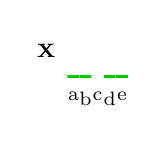
\begin{tikzpicture}
        \begin{axis}[
            ybar,
            axis y line=none,
            axis x line=bottom,
            axis line style={draw=none},
            ymin=0,
            ymax=100,
            width=2.2cm,
            height=2.2cm,
            bar width=1.5mm,
            xtick={a,b,c,d,e},
            xtick style={draw=none},
            symbolic x coords={a,b,c,d,e},
            xticklabel style={font=\scriptsize, anchor=north, yshift=-2pt},
            tick align=inside,
            enlarge x limits=0,
            clip=false,
        ]
            \addplot+[draw=none, fill=none, forget plot] coordinates {(e,100)};
            \addplot+[draw=green!80!black, very thick] coordinates {
            (a,0) (b,0) (d,0) (e,0)
            };

            % Label
            \node[
            anchor=south east,
            font=\scriptsize\bfseries,
            xshift=-1mm, yshift=-5mm
            ] at (current axis.north west) {X};

        \end{axis}
    \end{tikzpicture}
}

\newcommand{\blueCPY}{
    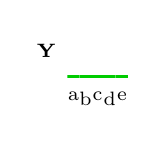
\begin{tikzpicture}
        \begin{axis}[
            ybar,
            axis y line=none,
            axis x line=bottom,
            axis line style={draw=none},
            ymin=0,
            ymax=100,
            width=2.2cm,
            height=2.2cm,
            bar width=1.5mm,
            xtick={a,b,c,d,e},
            xtick style={draw=none},
            symbolic x coords={a,b,c,d,e},
            xticklabel style={font=\scriptsize, anchor=north, yshift=-2pt},
            tick align=inside,
            enlarge x limits=0,
            clip=false,
        ]
            \addplot+[draw=none, fill=none, forget plot] coordinates {(e,100)};
            \addplot+[draw=green!80!black, very thick] coordinates {
            (a,0) (b,0) (c,0) (d,0) (e,0)
            };

            % Label
            \node[
            anchor=south east,
            font=\scriptsize\bfseries,
            xshift=-1mm, yshift=-5mm
            ] at (current axis.north west) {Y};

        \end{axis}
    \end{tikzpicture}
}

\newcommand{\blueCPZ}{
    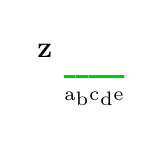
\begin{tikzpicture}
        \begin{axis}[
            ybar,
            axis y line=none,
            axis x line=bottom,
            axis line style={draw=none},
            ymin=0,
            ymax=100,
            width=2.2cm,
            height=2.2cm,
            bar width=1.5mm,
            xtick={a,b,c,d,e},
            xtick style={draw=none},
            symbolic x coords={a,b,c,d,e},
            xticklabel style={font=\scriptsize, anchor=north, yshift=-2pt},
            tick align=inside,
            enlarge x limits=0,
            clip=false,
        ]
            \addplot+[draw=none, fill=none, forget plot] coordinates {(e,100)};
            \addplot+[draw=green!80!black, very thick] coordinates {
            (a,0) (b,0) (c,0) (d,0) (e,0)
            };

            % Label
            \node[
            anchor=south east,
            font=\scriptsize\bfseries,
            xshift=-1mm, yshift=-5mm
            ] at (current axis.north west) {Z};

        \end{axis}
    \end{tikzpicture}
}

\newcommand{\redCPX}{
    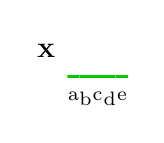
\begin{tikzpicture}
        \begin{axis}[
            ybar,
            axis y line=none,
            axis x line=bottom,
            axis line style={draw=none},
            ymin=0,
            ymax=100,
            width=2.2cm,
            height=2.2cm,
            bar width=1.5mm,
            xtick={a,b,c,d,e},
            xtick style={draw=none},
            symbolic x coords={a,b,c,d,e},
            xticklabel style={font=\scriptsize, anchor=north, yshift=-2pt},
            tick align=inside,
            enlarge x limits=0,
            clip=false,
        ]
            \addplot+[draw=none, fill=none, forget plot] coordinates {(e,100)};
            \addplot+[draw=green!80!black, very thick] coordinates {
            (a,0) (b,0) (c,0) (d,0) (e,0)
            };

            % Label
            \node[
            anchor=south east,
            font=\scriptsize\bfseries,
            xshift=-1mm, yshift=-5mm
            ] at (current axis.north west) {X};

        \end{axis}
    \end{tikzpicture}
}

\newcommand{\redCPW}{
    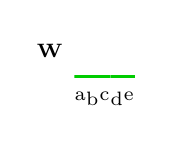
\begin{tikzpicture}
        \begin{axis}[
            ybar,
            axis y line=none,
            axis x line=bottom,
            axis line style={draw=none},
            ymin=0,
            ymax=100,
            width=2.2cm,
            height=2.2cm,
            bar width=1.5mm,
            xtick={a,b,c,d,e},
            xtick style={draw=none},
            symbolic x coords={a,b,c,d,e},
            xticklabel style={font=\scriptsize, anchor=north, yshift=-2pt},
            tick align=inside,
            enlarge x limits=0,
            clip=false,
        ]
            \addplot+[draw=none, fill=none, forget plot] coordinates {(e,100)};
            \addplot+[draw=green!80!black, very thick] coordinates {
            (a,0) (b,0) (c,0) (d,0) (e,0)
            };

            % Label
            \node[
            anchor=south east,
            font=\scriptsize\bfseries,
            xshift=-1mm, yshift=-5mm
            ] at (current axis.north west) {W};

        \end{axis}
    \end{tikzpicture}
}

\newcommand{\redCPZ}{
    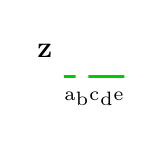
\begin{tikzpicture}
        \begin{axis}[
            ybar,
            axis y line=none,
            axis x line=bottom,
            axis line style={draw=none},
            ymin=0,
            ymax=100,
            width=2.2cm,
            height=2.2cm,
            bar width=1.5mm,
            xtick={a,b,c,d,e},
            xtick style={draw=none},
            symbolic x coords={a,b,c,d,e},
            xticklabel style={font=\scriptsize, anchor=north, yshift=-2pt},
            tick align=inside,
            enlarge x limits=0,
            clip=false,
        ]
            \addplot+[draw=none, fill=none, forget plot] coordinates {(e,100)};
            \addplot+[draw=green!80!black, very thick] coordinates {
            (a,0) (c,0) (d,0) (e,0)
            };

            % Label
            \node[
            anchor=south east,
            font=\scriptsize\bfseries,
            xshift=-1mm, yshift=-5mm
            ] at (current axis.north west) {Z};

        \end{axis}
    \end{tikzpicture}
}

% endregion


\begin{tikzpicture}[node distance=10pt and 20pt, thick]
    
    % Standard CP messaging
    \node (leftPicture) at (0,0) {
        \begin{tikzpicture}[node distance=10pt and 20pt, thick]
            \useasboundingbox (0,0) rectangle (5.5,2);
            % Left side: stacked bar plots with labels
            \matrix (left)[
                matrix of nodes,
                nodes={anchor=west},
                row sep=10pt,
                inner sep=0pt
            ] {
                \node {\blueCPX}; \\
                \node {\blueCPY}; \\ 
                \node {\blueCPZ}; \\
            };
            % Draw blue bounding box around left matrix
            \node[draw=blue, thick, inner sep=5pt, fit=(left)] (blueBox) {};
        
            % Right side: same matrix as left, shifted right of middle
            \matrix (right)[
                matrix of nodes,
                nodes={anchor=west},
                row sep=10pt,
                inner sep=0pt,
                right=4cm of left.center
            ] {
                \node {\redCPX}; \\
                \node {\redCPW}; \\
                \node {\redCPZ}; \\
            };
            % Draw red bounding box around left matrix
            \node[draw=red, thick, inner sep=5pt, fit=(right)] (redBox) {};
            
            \def\arrowSideGap{3mm}
            \def\arrowMidGap{0.75}
            \def\scale{0.75}
            \draw[->, thick]
                ([xshift=\arrowSideGap]blueBox.east |- 0, \arrowMidGap) --
                ([xshift=-\arrowSideGap]redBox.west |- 0, \arrowMidGap) 
                node[pos=0.25, above, yshift=-2mm] 
                {\textbf{X $\neq$ c}};
            \draw[->, thick]
                ([xshift=-\arrowSideGap]redBox.west |- 0, -\arrowMidGap) --
                ([xshift=\arrowSideGap]blueBox.east |- 0, -\arrowMidGap)
                node[pos=0.25, above, yshift=-2mm]
                {\textbf{Z $\neq$ b}};
        \end{tikzpicture}
    };
    
    % CPBP marginal messaging
    \node (rightPicture) [right=0mm of leftPicture.east] {
        \begin{tikzpicture}[node distance=10pt and 20pt, thick]
            \useasboundingbox (0,0) rectangle (5.5,2);
            % Left side: stacked bar plots with labels
            \matrix (left)[
                matrix of nodes,
                nodes={anchor=west},
                row sep=10pt,
                inner sep=0pt
            ] {
                \node {\blueGraphX}; \\
                \node {\blueGraphY}; \\ 
                \node {\blueGraphZ}; \\
            };
            % Draw blue bounding box around left matrix
            \node[draw=blue, thick, inner sep=5pt, fit=(left)] (blueBox) {};
        
            % Right side: same matrix as left, shifted right of middle
            \matrix (right)[
                matrix of nodes,
                nodes={anchor=west},
                row sep=10pt,
                inner sep=0pt,
                right=4cm of left.center
            ] {
                \node {\redGraphX}; \\
                \node {\redGraphW}; \\
                \node {\redGraphZ}; \\
            };
            % Draw red bounding box around left matrix
            \node[draw=red, thick, inner sep=5pt, fit=(right)] (redBox) {};
            
            \def\arrowSideGap{3mm}
            \def\arrowMidGap{0.75}
            \def\scale{0.75}
            \draw[->, thick]
                ([xshift=\arrowSideGap]blueBox.east |- 0, 1 + \arrowMidGap) --
                ([xshift=-\arrowSideGap]redBox.west |- 0, 1 + \arrowMidGap) 
                node[pos=0.25, above, yshift=-2mm] 
                {\scalebox{\scale}{\blueGraphX}};
            \draw[->, thick]
                ([xshift=-\arrowSideGap]redBox.west |- 0, \arrowMidGap) -- 
                ([xshift=\arrowSideGap]blueBox.east |- 0, \arrowMidGap)
                node[pos=0.25, above, yshift=-2mm]
                {\scalebox{\scale}{\redGraphX}};
            \draw[->, thick]
                ([xshift=\arrowSideGap]blueBox.east |- 0,-\arrowMidGap) --
                ([xshift=-\arrowSideGap]redBox.west |- 0,-\arrowMidGap)
                node[pos=0.25, above, yshift=-2mm]
                {\scalebox{\scale}{\blueGraphZ}};
            \draw[->, thick]
                ([xshift=-\arrowSideGap]redBox.west |- 0,-1 - \arrowMidGap) --
                ([xshift=\arrowSideGap]blueBox.east |- 0,-1 - \arrowMidGap)
                node[pos=0.25, above, yshift=-2mm]
                {\scalebox{\scale}{\redGraphZ}};
        \end{tikzpicture}
    };
    

\end{tikzpicture}

    }
    \caption[\acrlong{cpbp} messaging.]{Belief Propagation replaces standard constraint messages, which consist of a binary message indicating which values are supported in the domain, with a probabilistic distribution over the domain. As we can see, instead of communicating that the value $c$ for variable $X$ lacks a support, the blue constraint communicates that $X=c$ has a $0\%$ chance of being in a valid solution. This ensures that we can still communicate what values must be filtered out, but we also gain information on the other values in the domain.}
    \label{fig:cpbp_messaging}
\end{figure}

When multiple constraints interact on one variable, they each simultaneously communicate to the variable what they estimate the probability distribution to be. The variable then merges these probabilities into the final values as seen in Figure~\ref{fig:cpbp_combined}.



\begin{figure}[ht]
    \centering
    
% region CPBP bar graphs

% Bar graph representing the blue constraint's marginals on variable x
\newcommand{\emptyGraph}{
    \begin{tikzpicture}
        \begin{axis}[
            opacity=0,
            ybar,
            axis y line=none,
            axis x line=bottom,
            axis line style={draw=none},
            ymin=0,
            ymax=100,
            width=2.2cm,
            height=2.2cm,
            bar width=1.5mm,
            xtick={a,b,c,d,e},
            xtick style={draw=none},
            symbolic x coords={a,b,c,d,e},
            xticklabel style={font=\scriptsize, anchor=north, yshift=-2pt},
            axis x line=bottom,
            axis y line=left,
            tick align=inside,
            enlarge x limits=0,
            clip=false,
        ]
            \addplot+[draw=none, fill=none, forget plot] coordinates {(e,100)};
        \end{axis}
    \end{tikzpicture}
}

% Bar graph representing the blue constraint's marginals on variable y
\newcommand{\blueGraphY}{
    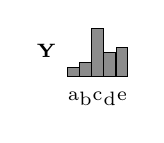
\begin{tikzpicture}
        \begin{axis}[
            ybar,
            axis y line=none,
            axis x line=bottom,
            axis line style={draw=none},
            ymin=0,
            ymax=100,
            width=2.2cm,
            height=2.2cm,
            bar width=1.5mm,
            xtick={a,b,c,d,e},
            xtick style={draw=none},
            symbolic x coords={a,b,c,d,e},
            xticklabel style={font=\scriptsize, anchor=north, yshift=-2pt},
            axis x line=bottom,
            axis y line=left,
            tick align=inside,
            enlarge x limits=0,
            clip=false,
        ]
            \addplot+[fill=gray!90, draw=black] coordinates {
                (a,20) (b,30) (c,100) (d,50) (e,60)
            };
            \node[
                anchor=south east,
                font=\scriptsize\bfseries,
                xshift=-1mm, yshift=-5mm
            ] at (current axis.north west) {Y};
        \end{axis}
    \end{tikzpicture}
}

% Bar graph representing the red constraint's marginals on variable w
\newcommand{\redGraphW}{
    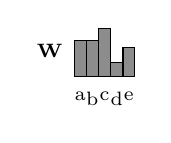
\begin{tikzpicture}
        \begin{axis}[
            ybar,
            axis y line=none,
            axis x line=bottom,
            axis line style={draw=none},
            ymin=0,
            ymax=100,
            width=2.2cm,
            height=2.2cm,
            bar width=1.5mm,
            xtick={a,b,c,d,e},
            xtick style={draw=none},
            symbolic x coords={a,b,c,d,e},
            xticklabel style={font=\scriptsize, anchor=north, yshift=-2pt},
            axis x line=bottom,
            axis y line=left,
            tick align=inside,
            enlarge x limits=0,
            clip=false,
        ]
            \addplot+[fill=gray!90, draw=black] coordinates {
                (a,75) (b,75) (c,100) (d,30) (e,60)
            };
            \node[
                anchor=south east,
                font=\scriptsize\bfseries,
                xshift=-1mm, yshift=-5mm
            ] at (current axis.north west) {W};
        \end{axis}
    \end{tikzpicture}
}

% Bar graph representing the combined marginals on variable x
\newcommand{\combinedX}{
    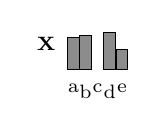
\begin{tikzpicture}
        \begin{axis}[
            ybar,
            axis y line=none,
            axis x line=bottom,
            axis line style={draw=none},
            ymin=0,
            ymax=100,
            width=2.2cm,
            height=2.2cm,
            bar width=1.5mm,
            xtick={a,b,c,d,e},
            xtick style={draw=none},
            symbolic x coords={a,b,c,d,e},
            xticklabel style={font=\scriptsize, anchor=north, yshift=-2pt},
            axis x line=bottom,
            axis y line=left,
            tick align=inside,
            enlarge x limits=0,
            clip=false,
        ]
            \addplot+[fill=gray!90, draw=black] coordinates {
                (a,65) (b,70) (d,75) (e,40)
            };
            \node[
                anchor=south east,
                font=\scriptsize\bfseries,
                xshift=-1mm, yshift=-5mm
            ] at (current axis.north west) {X};
        \end{axis}
    \end{tikzpicture}
}

% Bar graph representing the combined marginals on variable z
\newcommand{\combinedZ}{
    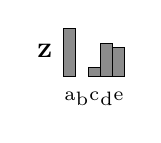
\begin{tikzpicture}
        \begin{axis}[
            ybar,
            axis y line=none,
            axis x line=bottom,
            axis line style={draw=none},
            ymin=0,
            ymax=100,
            width=2.2cm,
            height=2.2cm,
            bar width=1.5mm,
            xtick={a,b,c,d,e},
            xtick style={draw=none},
            symbolic x coords={a,b,c,d,e},
            xticklabel style={font=\scriptsize, anchor=north, yshift=-2pt},
            axis x line=bottom,
            axis y line=left,
            tick align=inside,
            enlarge x limits=0,
            clip=false,
        ]
            \addplot+[fill=gray!90, draw=black] coordinates {
                (a,100) (c,20) (d,69) (e,60)
            };
            \node[
                anchor=south east,
                font=\scriptsize\bfseries,
                xshift=-1mm, yshift=-5mm
            ] at (current axis.north west) {Z};
        \end{axis}
    \end{tikzpicture}
}

% endregion

    
\begin{tikzpicture}[node distance=10pt and 20pt, thick]
    % Left side: stacked bar plots with labels
    \matrix (left)[
        matrix of nodes,
        nodes={anchor=west},
        row sep=10pt,
        inner sep=0pt
    ] {
        \node {\emptyGraph}; \\
        \node {\blueGraphY}; \\ 
        \node {\emptyGraph}; \\
    };
    % Draw blue bounding box around left matrix
    \node[draw=blue, thick, inner sep=5pt, fit=(left)] (blueBox) {};

    % Right side: same matrix as left, shifted right of middle
    \matrix (right)[
        matrix of nodes,
        nodes={anchor=west},
        row sep=10pt,
        inner sep=0pt,
        right=4cm of left.center
    ] {
        \node {\emptyGraph}; \\
        \node {\redGraphW}; \\
        \node {\emptyGraph}; \\
    };
    % Draw red bounding box around left matrix
    \node[draw=red, thick, inner sep=5pt, fit=(right)] (redBox) {};
    
    % Right side: same matrix as left, shifted right of middle
    \matrix (middle)[
        matrix of nodes,
        nodes={anchor=west},
        row sep=10pt,
        inner sep=0pt,
        right=1.5cm of left.center
    ] {
        \node {\combinedX}; \\
        \node {\emptyGraph}; \\
        \node {\combinedZ}; \\
    };

    \node[draw=green, dashed, inner sep=5pt, fit=(left)(right)] (greenBox) {};
\end{tikzpicture}

    \caption[\acrlong{cpbp} combining probabilities]{The variables which are affected by multiple constraints ($X$ and $Z$) merge the communicated probabilities that were communicated by the different constraints. $X$ filters out the value $c$ and $Z$ filters out $b$, as was communicated by the constraints seen in Figure~\ref{fig:cpbp_messaging}.}
    \label{fig:cpbp_combined}
\end{figure}

\subsection{Among Constraint}

\subsection{Element Constraint}

\subsection{Grammar Constraint}

\subsection{Regular Constraint}

\subsection{Sum Constraint}

\subsection{Table Constraint}
\subsubsection{Short Table Constraint}


\end{document}